\subsection{SGX Software Attestation}
\label{sec:sgx_attestation}

The software attestation scheme implemented by SGX follows the principles
outlined in \S~\ref{sec:generic_software_attestation}. An SGX-enabled processor
computes a measurement of the code and data that is loaded in each enclave,
which is similar to the measurement computed by the TPM~(\S~\ref{sec:tpm}). The
software inside an enclave can start a process that results in an SGX
attestation signature, which includes the enclave's measurement and an enclave
message.

\begin{figure}[hbt]
  \centering
  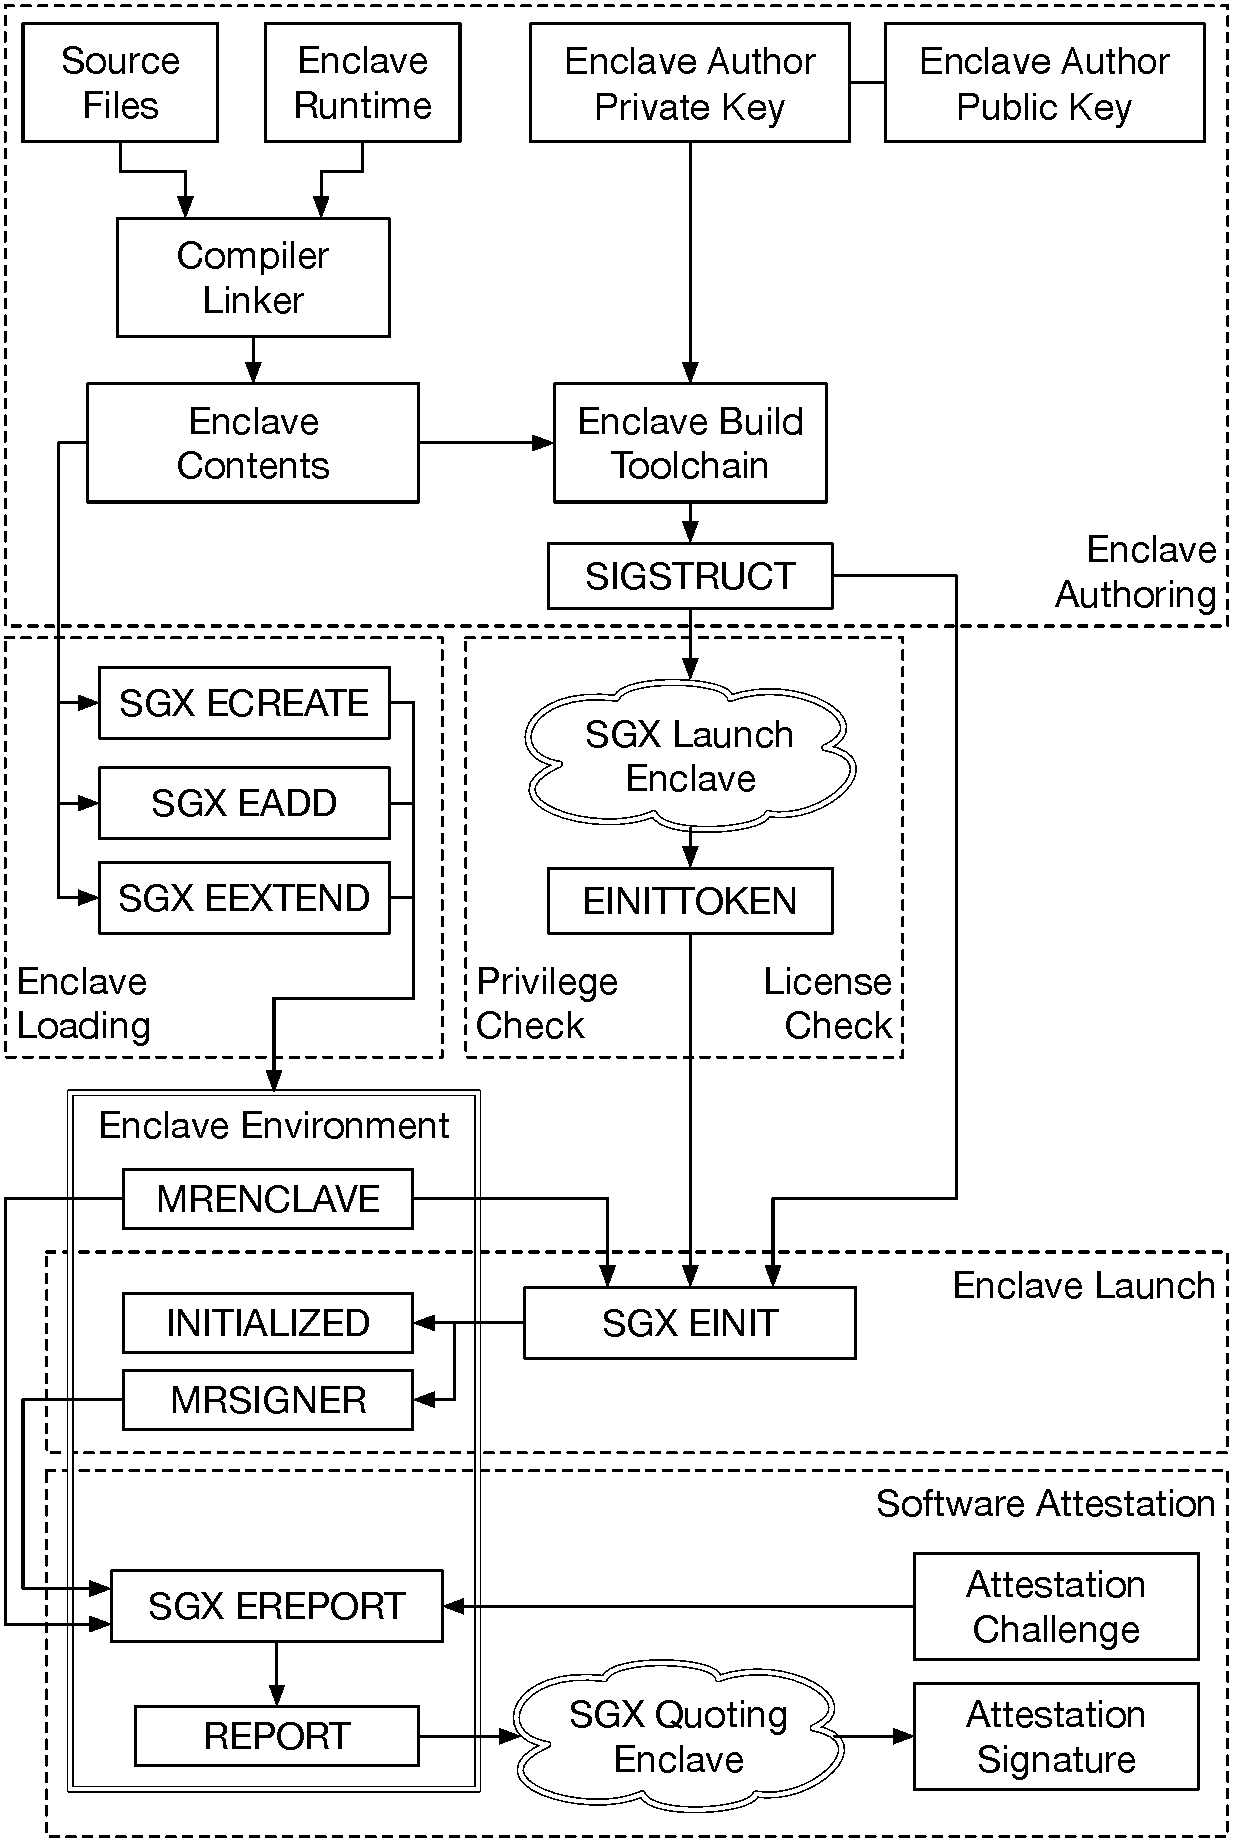
\includegraphics[width=85mm]{figures/sgx_attestation_overview.pdf}
  \caption{
    Setting up an SGX enclave and undergoing the software attestation process
    involves the SGX instructions \texttt{EINIT} and \texttt{EREPORT}, and two
    special enclaves authored by Intel, the SGX Launch Enclave and the SGX
    Quoting Enclave.
  }
  \label{fig:sgx_attestation_overview}
\end{figure}

% EPID signing takes too long for microcode.
%   US 8,972,746 B2 - 21:8-16, 33:16-29, 33:58

The cryptographic primitive used in SGX's attestation signature is too complex
to be implemented in hardware, so signing process is performed by a privileged
\textit{Quoting Enclave}, which is issued by Intel, and can access the SGX
attestation key. This enclave is discused in \S~\ref{sec:sgx_quoting_enclave}.

Pushing the signing functionality into the Quoting Enclave creates the need for
a secure communication path between an enclave that desires to undergo
software attestation and the Quoting Enclave. The SGX design solves this
problem with a local attestation mechanism that can be used by an enclave to
prove its identity to any other enclave hosted by the same SGX-enabled CPU.
This scheme, described in \S~\ref{sec:sgx_ereport}, is implemented by the
\texttt{EREPORT} instruction.

% Keys: SDM S 39.4.3
% ISCA SGX Slides 104, 105, 106

The SGX attestation key used by the Quoting Enclave does not exist at the time
SGX-enabled processors leave the factory. The attestation key is provisioned
later, using a largely undocumented process that is known to involve at least
one other enclave issued by Intel, and at least two special \texttt{EGETKEY}
key types. The publicly available details of this process are summarized in
\S~\ref{sec:sgx_quoting_enclave}.

The SGX implementation contained in a CPU's hardware does not directly enforce
the enclave attribute checks that decide which enclaves can access the CPU
secrets used for software attestation. The potentially complex restrictions on
enclave attributes are instead enforced by the Launch Enclave, which is an
enclave issued by Intel that gets to approve every other enclave before it is
initialized by \textit{EINIT}~(\S~\ref{sec:sgx_einit_overview}). The officially
documented information about the approval process is discussed in
\S~\ref{sec:sgx_launch_enclave}.

% Enclave License
%   US 8,972,746 B2 - 34:6-23
% Licenses are evaluated into Permits (which became EINITTTOKEN)
%   US 8,972,746 B2 - 34:24-29, 35:27-59
% EINIT requires a Permit to launch a production enclave
%   US 8,972,746 B2 - 35:60-67, 36:1-3, 36:47-52, 38:4-65
% License Enclave creates Permit
%   US 8,972,746 B2 - 36:40-46, 37:50-67, 38:1-3
% EMKPERMIT seems to have gotten merged into EINIT
%   US 8,972,746 B2 - 36:53-67, 37:1-7, 37:24-49
% License became SIGSTRUCT
%   US 8,972,746 B2 - 37:8-23

The SGX patents~\cite{intel2013patent1, intel2013patent2} disclose in no
uncertain terms that the Launch Enclave was introduced to ensure that each
enclave's author has a business relationship with Intel, and implements a
software licensing system. \S~\ref{sec:sgx_licensing} briefly discusses the
implications, should this turn out to be true.


\subsubsection{Local Attestation}
\label{sec:sgx_ereport}

% Using REPORTs for Local Attestation: SDM S 39.4.3.2
% EREPORT: SDM S 41.4.1

An enclave proves its identity to another \textit{target enclave} via the
\texttt{EREPORT} instruction shown in Figure~\ref{fig:sgx_ereport}. The SGX
instruction produces an attestation \textit{Report} (REPORT) that
cryptographically binds a message supplied by the enclave with the enclave's
measurement-based~(\S~\ref{sec:sgx_measurement}) and
certificate-based~(\S~\ref{sec:sgx_certificate_identity}) identities. The
cryptographic binding is accomplished by a MAC
tag~(\S~\ref{sec:integrity_crypto}) computed using a symmetric key that is only
shared between the target enclave and the SGX implementation.

\begin{figure}[hbt]
  \centering
  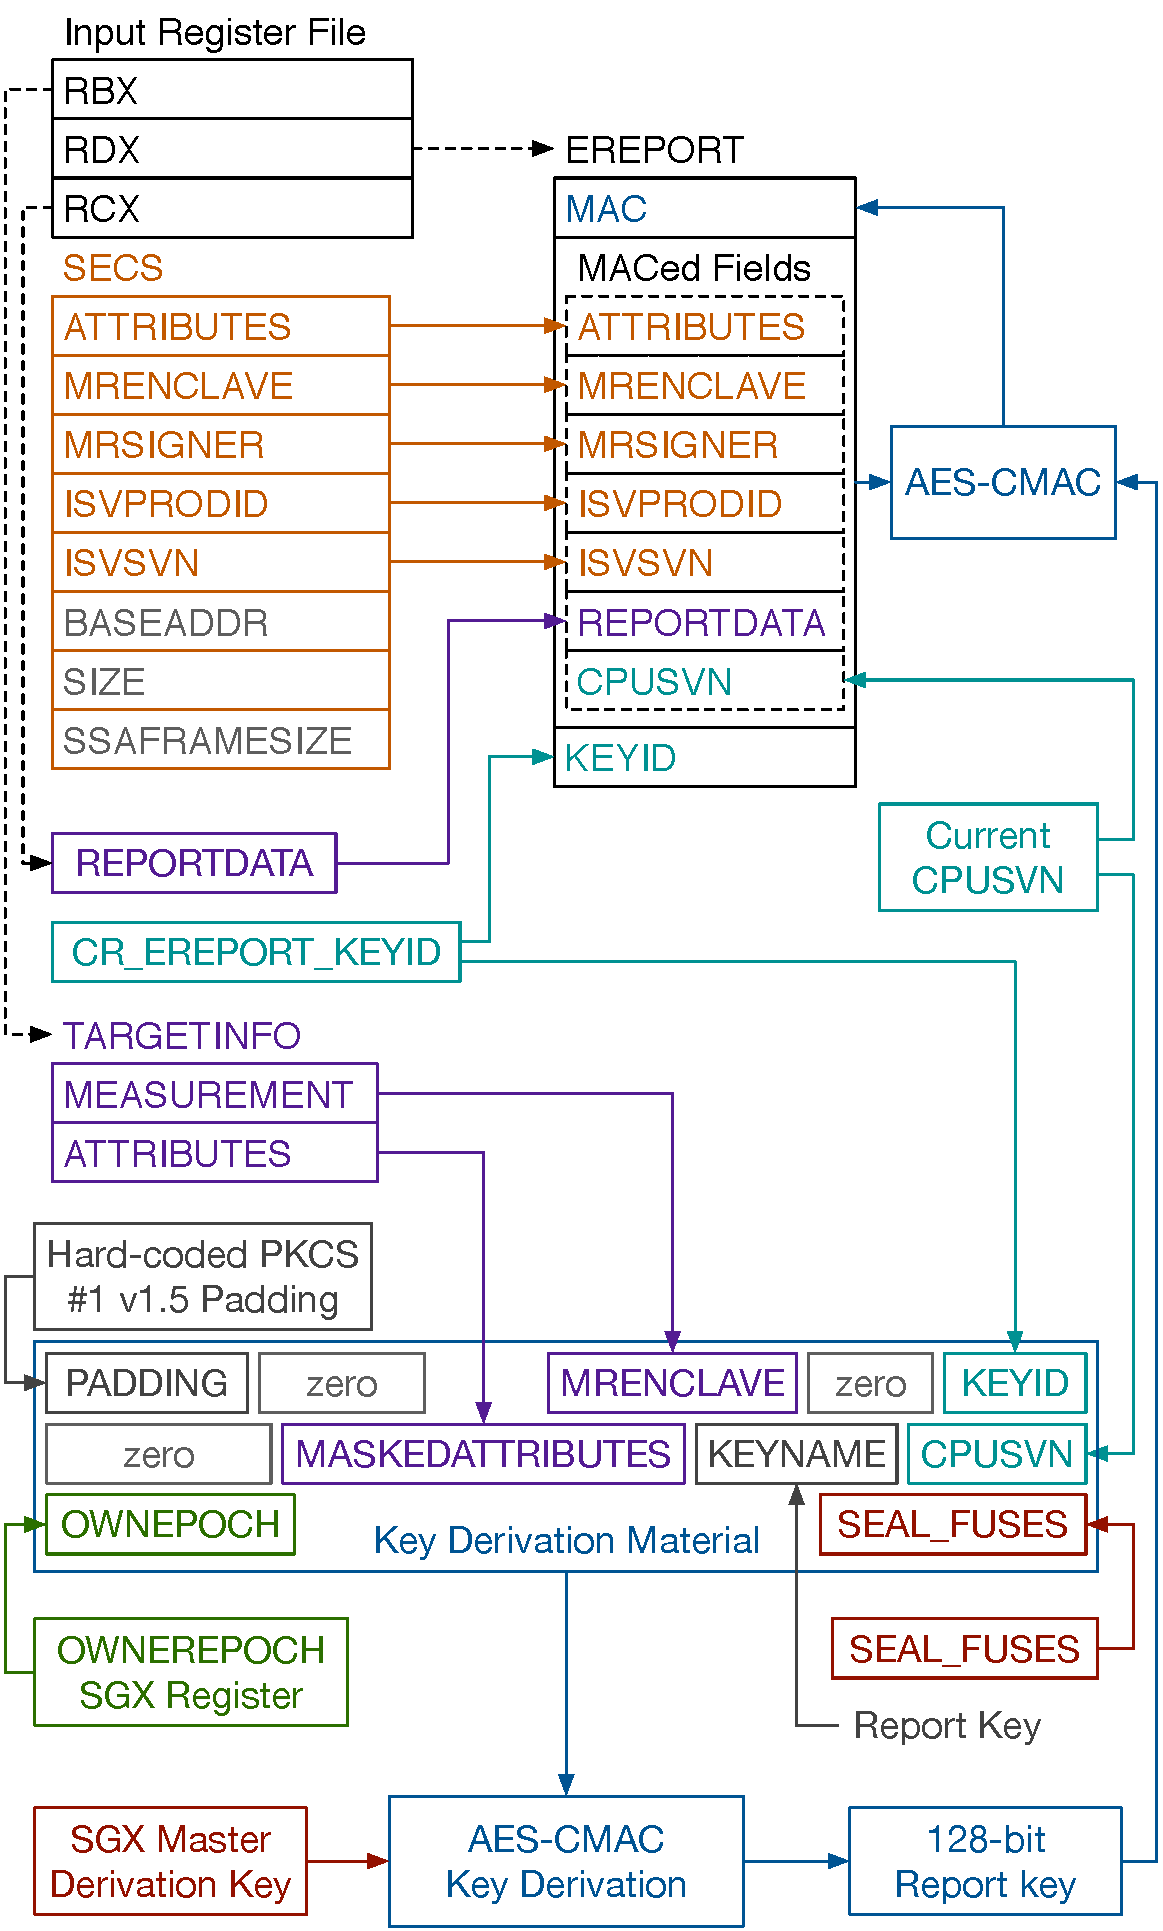
\includegraphics[width=85mm]{figures/sgx_ereport.pdf}
  \caption{
    \texttt{EREPORT} data flow
  }
  \label{fig:sgx_ereport}
\end{figure}

The \texttt{EREPORT} instruction reads the current enclave's identity
information from the enclave's SECS~(\S~\ref{sec:sgx_secs}), and uses it to
populate the REPORT structure. Specifically, \texttt{EREPORT} copies the
SECS fields indicating the enclave's measurement (MRENCLAVE), certificate-based
identity (MRSIGNER, ISVPROD, ISVSVN), and attributes (ATTRIBUTES). The
attestation report also includes the SVN of the SGX implementation (CPUSVN)
and a 64-byte (512-bit) message supplied by the enclave.

% Keys: SDM S 39.4.3

The target enclave that receives the attestation report can convince itself of
the report's authenticy as shown in Figure~\ref{fig:sgx_ereport_check}. The
report's authenticity proof is its MAC tag. The key required to verify the MAC
can only be obtained by the target enclave, by asking
\texttt{EGETKEY}~(\S~\ref{sec:sgx_egetkey}) to derive report key. The SDM
states that the MAC tag is computed using a block cipher-based
MAC~(CMAC,~\cite{fips2005cmac}), but stops short of specifying the underlying
cipher. One of the SGX papers~\cite{anati2013sgx} states that the CMAC is based
on 128-bit AES.

\begin{figure}[hbt]
  \centering
  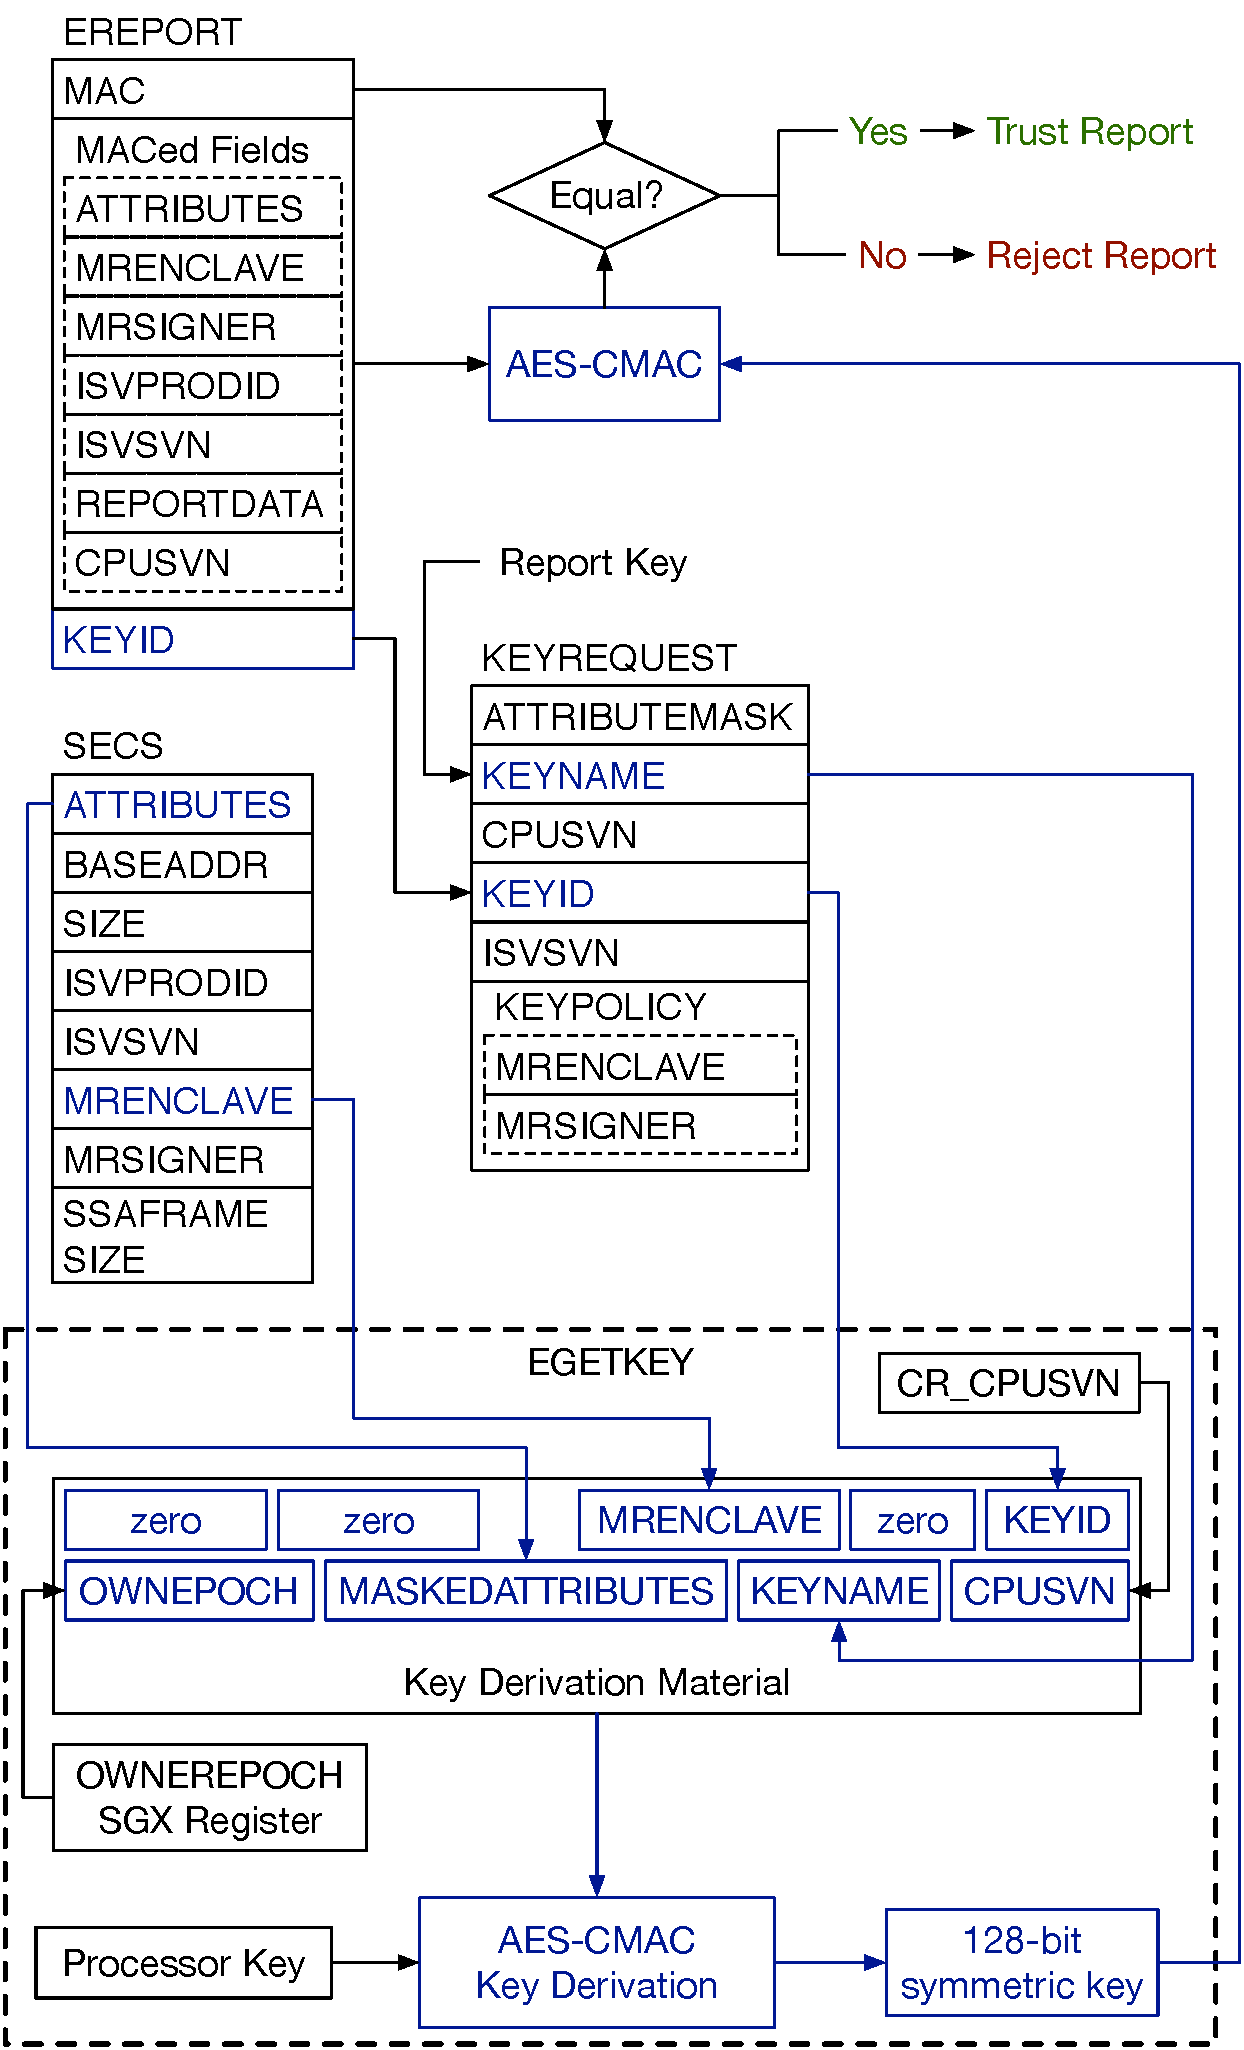
\includegraphics[width=87mm]{figures/sgx_ereport_check.pdf}
  \caption{
    The authenticty of the REPORT structure created by \texttt{EREPORT} can and
    should be verified by the report's target enclave. The target's code uses
    \texttt{EGETKEY} to obtain the key used for the MAC tag embedded in the
    REPORT structure, and then verifies the tag.
  }
  \label{fig:sgx_ereport_check}
\end{figure}

The report key returned by \texttt{EGETKEY} is derived from a secret embedded
in the processor~(\S~\ref{sec:sgx_egetkey}), and the key material includes the
target enclave's measurement. The target enclave can be assured that the MAC
tag in the report was produced by the SGX implementation, for the following
reasons. The cryptographic properties of the underlying key derivation and
MAC algorithms ensure that only the SGX implementation can produce the MAC tag,
as it is the only entity who can access the processor's secret, and it would be
impossible for an attacker to derive the report key without knowing the
processor's secret. The SGX design guarantees that the key produced by
\texttt{EGETKEY} depends on the calling enclave's measurement, so only the
target enclave can obtain the key used to produce the MAC tag in the report.

\texttt{EREPORT} uses the same key derivation process as \texttt{EGETKEY}
does when invoked with KEYNAME set to the value associated with report keys.
For this reason, \texttt{EREPORT} requires the virtual address of a
\textit{Report Target Info}~(TARGETINFO) structure that contains the
measurement-based identity and attributes of the target enclave.

% EGETKEY: SDM S 41.4.1
% Key Derivation: SDM Table 41-43

When deriving a report key, \texttt{EGETKEY} behaves slightly differently than
it does in the case of seal keys, as shown in
Figure~\ref{fig:sgx_ereport_check}. The key generation material never includes
the fields corresponding to the enclave's certificate-based identity (MRSIGNER,
ISVPRODID, ISVSVN), and the KEYPOLICY field in the KEYREQUEST structure is
ignored. It follows that the report can only be verified by the target enclave.

Furthermore, the SGX implementation SVN~(CPUSVN) value used for key generation
is determined by the current CPUSVN, instead from being read from the Key
Request structure. Therefore, SGX implementation upgrades that increase the
CPUSVN invalidate all outstanding reports. Given that CPUSVN increases are
associated with security fixes, the argument in
\S~\ref{sec:sgx_certificate_identity} suggests that this restriction may reduce
the impact of vulnerabilities in the SGX implementation.

Last, \texttt{EREPORT} sets the KEYID field in the key generation material to
the contents of an SGX configuration register (CR\_REPORT\_KEYID) that is
initialized with a random value when SGX is initialized. The KEYID value is
also saved in the attestation report, but it is not covered by the MAC tag.

% EREPORT key derivation
%   US 8,972,746 B2 - 21:51-67, 22:1-6, Figure 12
% EREPORT uses KeyID which is incremented after 2^32 AES operations
%   US 8,972,746 B2 - 22:7-12
% EREPORT's MAC is actually a GMAC, not a CMAC
%   US 8,972,746 B2 - 21:64-67


\subsubsection{Remote Attestation}
\label{sec:sgx_quoting_enclave}

The SDM paints a complete picture of the local attestation mechanism that was
described in \S~\ref{sec:sgx_ereport}. In comparison, the remote attestation
process, which includes the Quoting Enclave and the underlying keys, is
shrouded in mistery. This section presents the information that can be gleaned
from the SDM and in the ISCA 2015 SGX tutorial~\cite{intel2015iscasgx}.

% Keys: SDM S 39.4.3
% ISCA SGX Slides 104, 105, 106
% ISCA SGX Slide 105:
%   "Intel generates and fuses a unique key during manufacturing"
%   "Intel maintains a database of these keys."

SGX's software attestation scheme, which is illustrated in
Figure~\ref{fig:sgx_attestation_keys}, relies on a key generation facility and
on a provisioning service, both operated by Intel.

\begin{figure}[hbt]
  \centering
  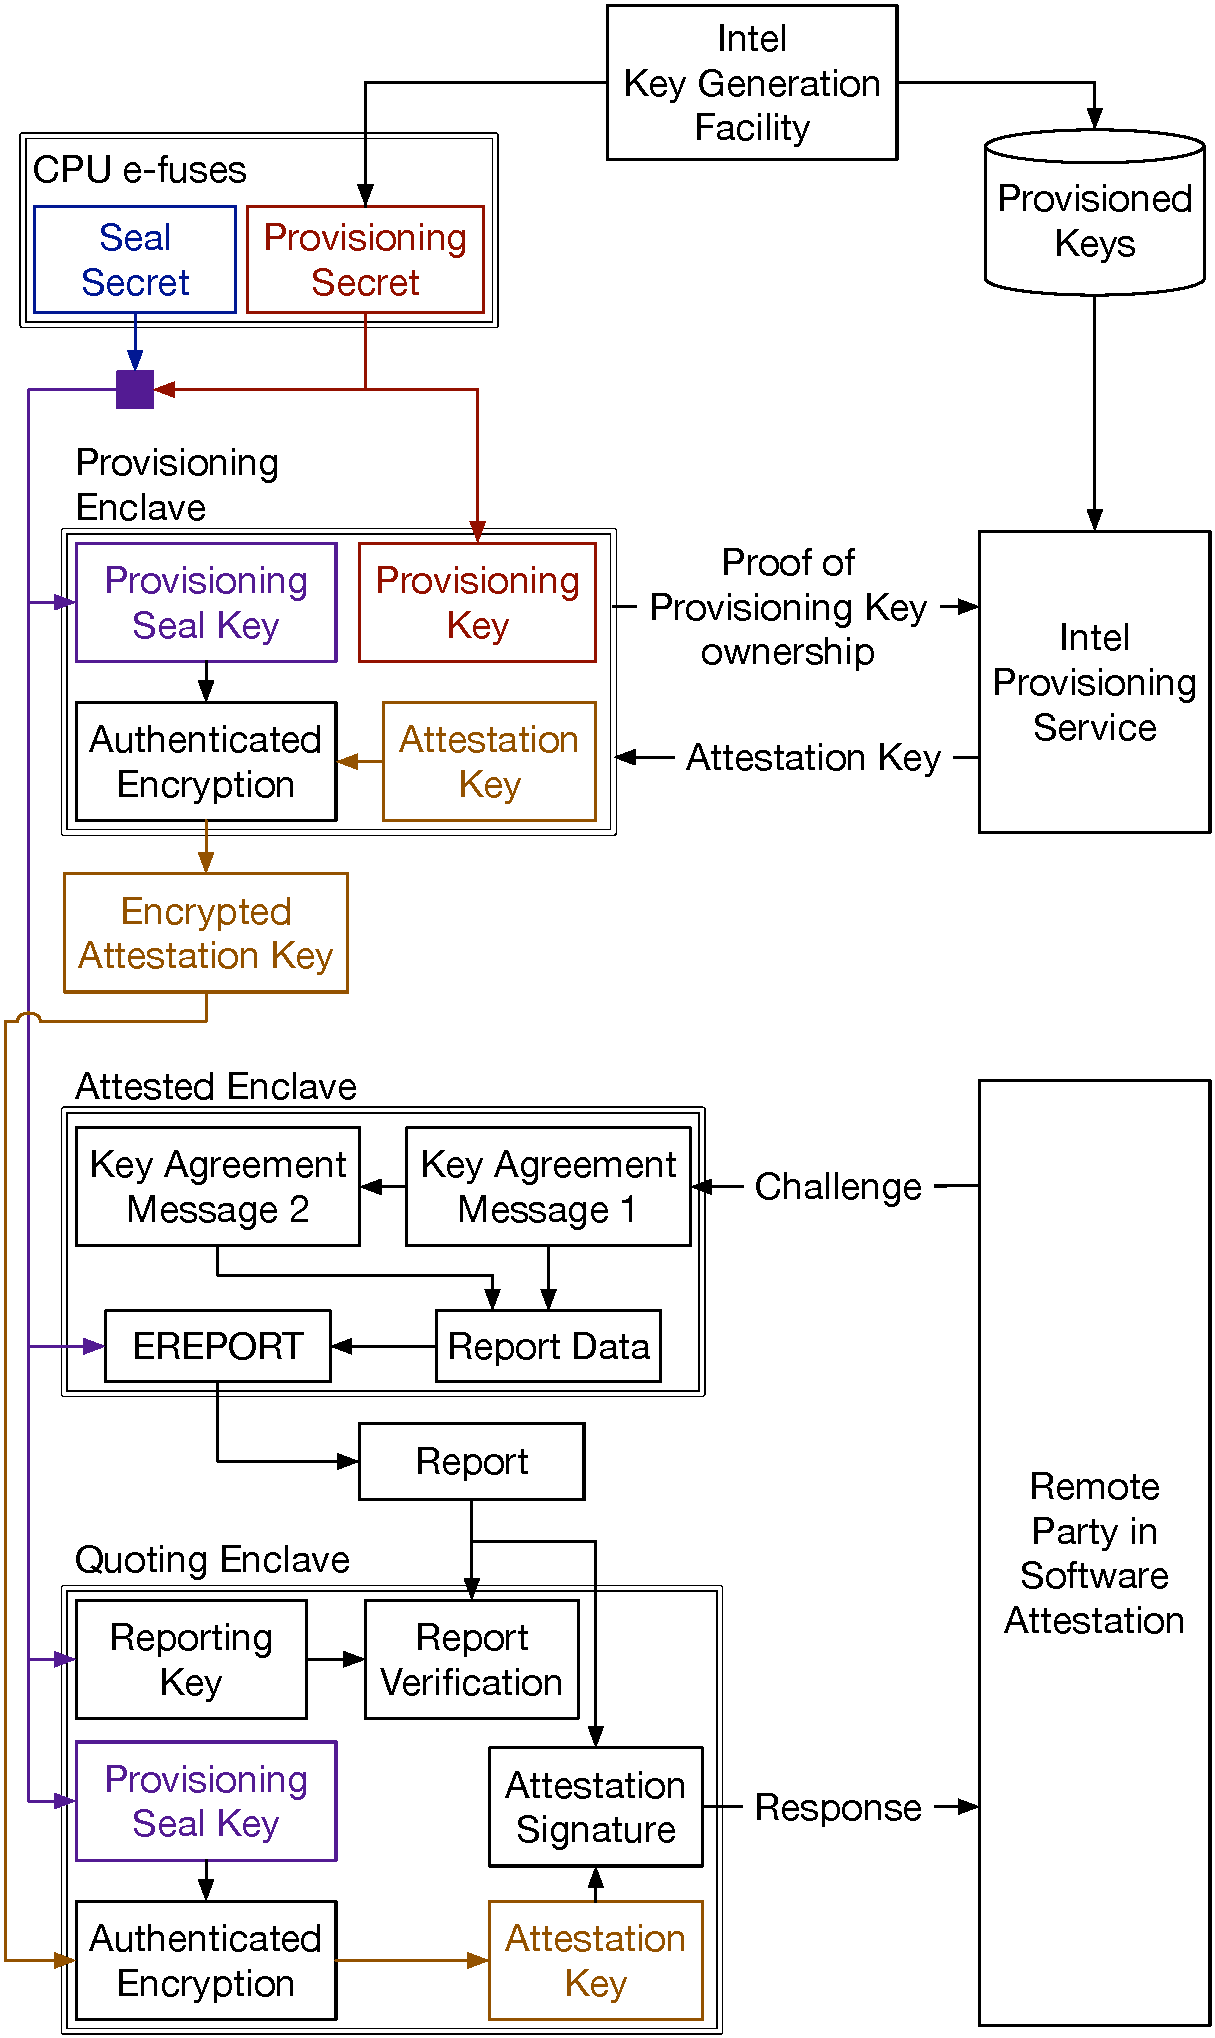
\includegraphics[width=85mm]{figures/sgx_attestation_keys.pdf}
  \caption{
    SGX's software attestation is based on two keys in the processor's e-fuses,
    and on a key received from Intel's provisioning service.
  }
  \label{fig:sgx_attestation_keys}
\end{figure}

During the manufacturing process, an SGX-enabled processor communicates with
Intel's key generation facility, and has two keys burned into its e-fuses. We
shall refer to these keys as the \textit{Fused Seal Key} and the
\textit{Provisioning Key}. .

% EGETKEY: SDM S 41.4.1
% Key Derivation: SDM Table 41-43

The Fused Seal Key never leaves the CPU, and is only used by \texttt{EGETKEY}
as the master key for the key derivation service that it provides. The Fused
Seal Key is the ``Processor Key'' in Figures \ref{fig:sgx_egetkey},
\ref{fig:sgx_attestation_overview}, \ref{fig:sgx_ereport}, and
\ref{fig:sgx_ereport_check}. The pseudocode in the SDM uses the CR\_SEAL\_FUSES
register name to refer to the location that stores the Fused Seal Key.

The name Fused Seal Key deviates slightly from Intel's official documentation.
Intel's documents confusingly use the ``Seal Key'' name to refer to both the
key stored in e-fuses, which is introduced here, and to one of the keys derived
by \texttt{EGETKEY}, which was described in \S~\ref{sec:sgx_egetkey}

The Provisioning Key can be accessed via \texttt{EGETKEY} by enclaves whose
PROVISIONKEY attribute is set to true. It is used by a Provisioning Enclave,
which is issued by Intel, to authenticate the SGX-enabled CPU to Intel's
provisioning service.

After the Provisioning Enclave proves the knowledge of the Provisioning Key to
Intel's provisioning service, the service generates an \textit{Attestation Key}
and sends it to the Provisioning Enclave. The enclave then encrypts the
Attestation Key using the \textit{Provisioning Seal Key}, and hands off the
encrypted key to the system software for storage.

The Provisioning Seal Key is obtained using the key derivation service
implemented by \texttt{EGETKEY}, and is only accessible to enclaves with the
PROVISIONKEY attribute. As its name suggests, the key is derived in a very
similar manner to the Seal Keys~(\S~\ref{sec:sgx_egetkey}) used to migrate
secrets between enclaves. The main difference between the Provisioning Seal Key
and regular Seal Keys is that the former is derived without using OWNEREPOCH,
so that the encrypted attestation key can be decrypted even if the CPU changes
owners.

After the provisioning steps above have been completed, the Quoting Enclave can
be invoked to perform SGX's software attestation. This enclave receives local
attestation reports~(\S~\ref{sec:sgx_ereport}) and verifies them using the
report keys generated by \texttt{EGETKEY}. The Quoting Enclave then obtains
the Provisioning Seal Key from \texttt{EGETKEY} and uses it to decrypt the
Attestation Key, which is received from system software. Last, the enclave
uses the Attestation Key to sign the information in the local attestation
report, producing an \textit{Attestation Signature}.

% Quoting Enclave is a reference to the TPM
%   US 8,972,746 B2 - 20:59-67

The SGX patents state that the name ``Quoting Enclave'' was chosen as a
reference to the TPM~(\S~\ref{sec:tpm})'s quoting feature, which is used to
perform software attestation on a TPM-based system.

The Attestation Key uses Intel's \textit{Enhanced Privacy ID}~(EPID)
cryptosystem~\cite{brickell2009epid}, which is a group signature scheme that is
intended to preserve the anonimity of the signer. Analyzing the correctness of
cryptographic schemes such as EPID, is outside the scope of this work, even
though the security of SGX hinges on EPID.

It is somewhat troubling that our description here contradicts the contents of
the SGX patents~\cite{intel2013patent1, intel2013patent2}. The patents state
that each SGX processor has an EPID key called the Device Attestation Key~(DAK)
burned in its fuses. The DAK can be used to produce attestation signatures as
soon as the processor leaves the factory, without the need to communicate with
any online service. According to the patents, Intel's provisioning service is
only used to re-prosivion keys when the DAK is revoked.

The picture painted by the SGX patents is more enticing, as it entails more
anonymity for the owners of SGX-enabled processors. Using EPID for the DAK
means that Intel's provisioning service never has the ability to track
individual processor chips.

This work always chooses to trust the information in official documentation
over patents, as the lengthy timelines associated with patent applications
means that patents are likely to represent an early version of the SGX design.
Therefore, we assume that Figure~\ref{fig:sgx_attestation_keys} paints an
accurate picture of the key usage in SGX's software attestation, which entails
that Intel can trace each attestation key to a specific piece of silicon.


\subsubsection{Enclave Attributes Access Control}
\label{sec:sgx_launch_enclave}

% ATTRIBUTES: SDM S 38.7.1

The security of SGX's software attestation scheme depends on denying
unauthorized enclaves access to the provisioning
keys~(\S~\ref{sec:sgx_quoting_enclave}) that can be used to obtain an
Attestation Key. This requirement translates into only allowing the
PROVISIONKEY attribute to be set for the enclaves that are trusted to carry out
the attestation process.

The logic embedded in the circuitry of SGX-enabled processors does not directly
control the use of the PROVISIONKEY attribute. Instead, the SGX design requires
that all enclaves be vetted by a \textit{Launch Enclave}~(LE) that implements
the access control checkes needed for the PROVISIONKEY attribute, and for any
other privileged attributes that may be introduced in future designs.

The LE is only briefly mentioned in Intel's official documentation. Neither its
behavior nor its interface with the system software is specified. We speculate
that Intel has not been forthcoming about the LE because of its role in
enforcing software licensing, which will be discussed in
\S~\ref{sec:sgx_licensing}. This section ignores the licensing aspect, and
describes a minimal LE implementation, illustrated in
Figure~\ref{fig:sgx_einittoken}, which would satisfy SGX's security
requirements.

\begin{figure}[hbt!]
  \centering
  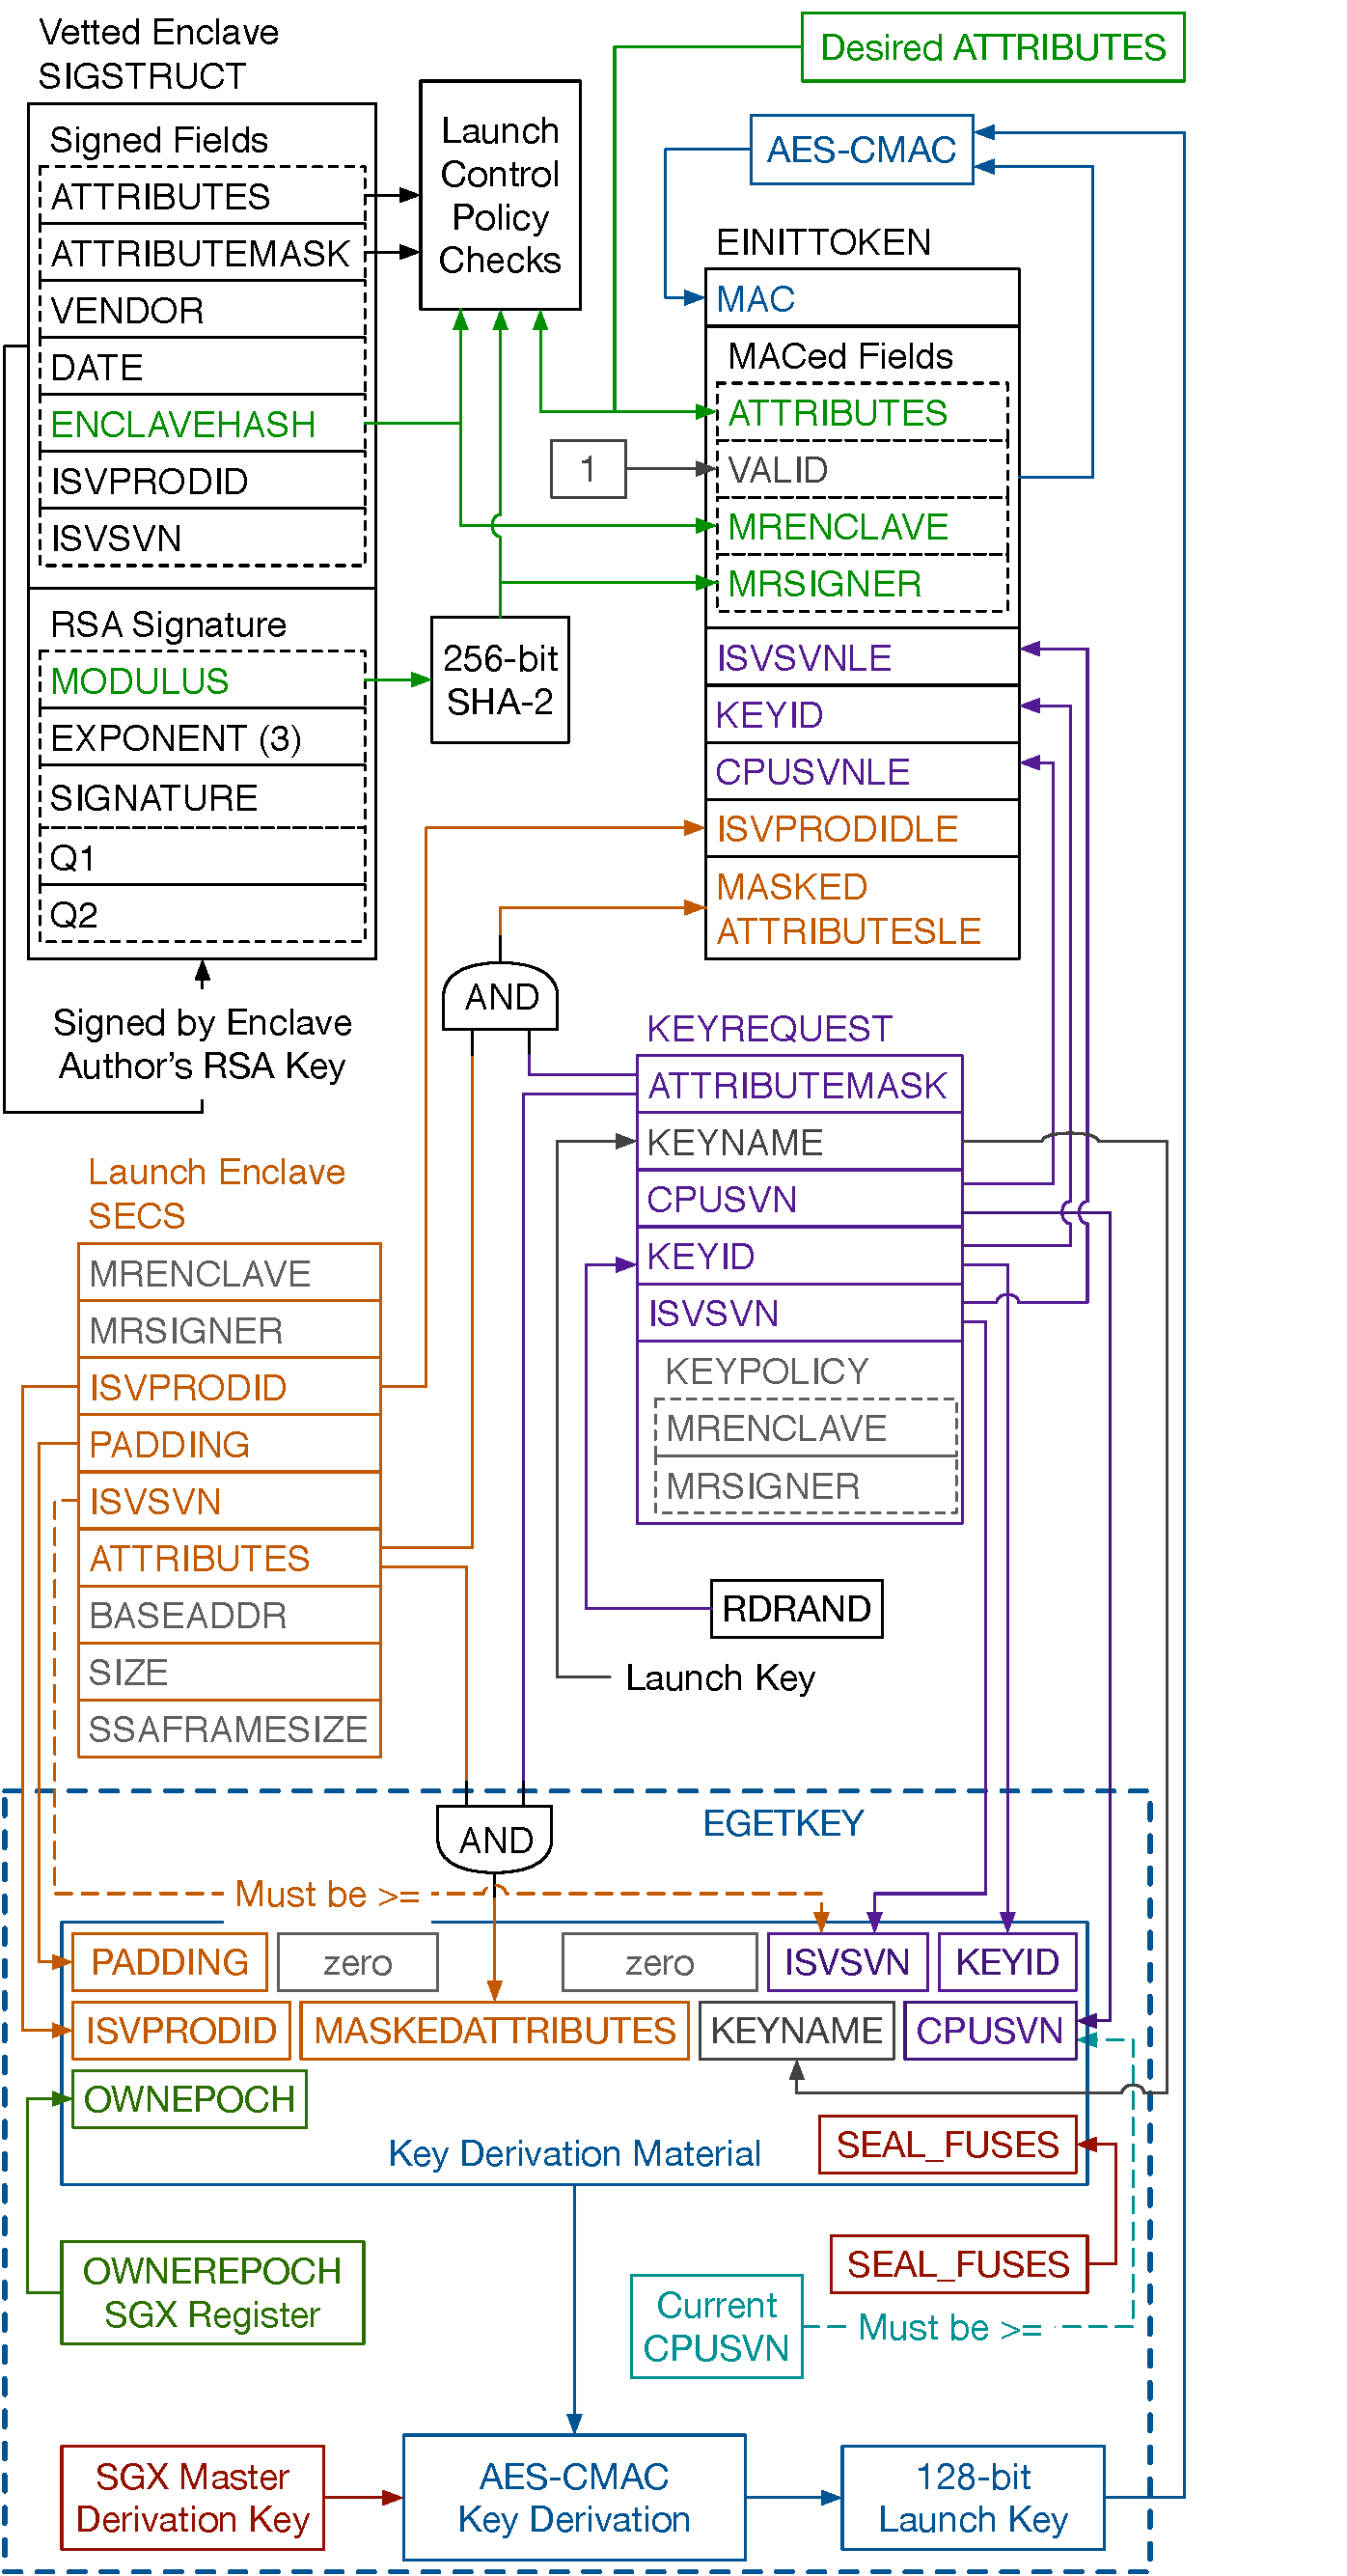
\includegraphics[width=95mm]{figures/sgx_einittoken.pdf}
  \caption{
    The SGX Launch Enclave computes the EINITTOKEN.
  }
  \label{fig:sgx_einittoken}
\end{figure}

% EINIT Token Structure (EINITTOKEN): SDM S 38.14

The LE approves an enclave by issuing an \textit{EINIT Token}~(EINITTOKEN) that
contains the approved enclave's
measurement-based~(\S~\ref{sec:sgx_measurement})
and certificate-based~(\S~\ref{sec:sgx_certificate_identity}) identities, just
like a local attestation REPORT~(\S~\ref{sec:sgx_ereport}). This token is
inspected by \texttt{EINIT}~(\S~\ref{sec:sgx_einit_overview}), which refuses to
initialize enclaves with incorrect tokens.

While an EINIT token is handled by untrusted system software, its integrity is
protected by a MAC tag~(\S~\ref{sec:integrity_crypto}) that is computed using a
\textit{Launch Key} obtained from \texttt{EGETKEY}. The \texttt{EINIT}
implementation follows the same key derivation process as \texttt{EGETKEY} to
convince itself that the EINITTOKEN provided to it was indeed generated by an
LE that had access to the Launch Key.

The SDM does not document the MAC algorithm used to confer integrity guarantees
to the EINITTOKEN structure. However, the \texttt{EINIT} pseudocode verifies
the token's MAC tag using same function that the \textit{EREPORT} pseudocode
uses to create the REPORT structure's MAC tag. It follows that the reasoning in
\S~\ref{sec:sgx_ereport} can be reused to conclude that EINITTOKEN structures
are MACed using AES-CMAC with 128-bit keys.

% EGETKEY: SDM S 41.4.1
% Key Derivation: SDM Table 41-43

The \texttt{EGETKEY} instruction only derives the Launch Key for enclaves that
have the LAUNCHKEY attribute set to true. The Launch Key is using the same
process as the Seal Key~(\S~\ref{sec:sgx_egetkey}). The derivation material
includes the current enclave's versioning information (ISVPRODID and ISVSVN)
but it does not include the main fields that convey an enclave's identity,
which are MRSIGNER and MRENCLAVE. The rest of the derivation material follows
the same rules as the material used for Seal Keys.

The EINITTTOKEN structure contains the identities of the approved enclave
(MRENCLAVE and MRSIGNER) and the approved enclave attributes (ATTRIBUTES). The
token also includes the information used for the Launch Key derivation,
which includes the LE's Product ID (ISVPRODIDLE), SVN (ISVSVNLE), and the
bitwise AND between the LE's ATTRIBUTES and the ATTRIBUTEMASK used in the
KEYREQUEST (MASKEDATTRIBUTESLE).

The EINITTOKEN information used to derive the Launch Key can also be used
by \texttt{EINIT} for damage control, e.g. to reject tokens issued by Launch
Enclaves with known security vulnerabilities. The reference pseudocode supplied
in the SDM states that \texttt{EINIT} checks the DEBUG bit in the
MASKEDATTRIBUTESLE field, and will not initialize a production enclave using
a token issued by a debugging LE. It is worth noting that MASKEDATTRIBUTESLE is
guaranteed to include the LE's DEBUG attribute, because \texttt{EGETKEY} forces
the DEBUG attribute's bit in the attributes mask to 1
(\S~\ref{sec:sgx_egetkey}).

The check described above makes it safe for Intel's privileged key to sign
Launch Enclaves with debugging features enabled. Without this check, using a
privileged Intel signing key on a single debug LE could invalidate SGX's
security guarantees on all the CPU chips that accept that signing key.
Concretely, if the issued SIGSTRUCT would be leaked, any attacker could build a
debugging LE, use the SGX debugging features to modify the code inside it, and
issue tokens that authorize malicious enclaves to access the Provisoning Key
used by the software attestation process.

A further advantage of the check described above is that Intel can supply SGX
enclave developers with a debugging LE that performs minimal or no security
checks before issuing an EINITTOKEN. The debugging LE can be used to launch any
enclave with the DEBUG attribute set. The DEBUG attribute is always included in
\texttt{EGETKEY}'s key derivation material, so debugging enclaves cannot access
the symmetric keys used to encrypt the secrets of production enclaves.

% EINIT: SDM S 41.3
% EINITTOKENKEY is bit 5, INTEL_ONLY_MASK is 0x20

The enclave attributes access control system described above relies on the LE
to reject initialization requests that set privileged attributes such as
PROVISIONKEY on unauthorized enclaves. However, the LE cannot vet itself, as
there will be no LE available when the LE itself needs to be initialized.
Therefore, the Launch Key access restrictions are implemented in hardware.

\texttt{EINIT} accepts an EINITTOKEN whose VALID bit is set to zero, if
the enclave's MRSIGNER~(\S~\ref{sec:sgx_mrsigner}) equals a hard-coded value
that corresponds to an Intel public key. For all other enclave authors, an
invalid EINIT token causes \texttt{EINIT} to reject the enclave and produce an
error code.

This exemption to the token verification policy provides a way to bootstrap the
enclave attributes access control system, namely using a zeroed out EINITTOKEN
to initialize the Launch Enclave. At the same time, the cryptographic
primitives behind the MRSIGNER check guarantee that only Intel-provided
enclaves will be able to bypass the attribute checks. This does not change
SGX's security properties because Intel is already a trusted party, as it is
responsible for generating the Provisioning Keys and Attestation Keys used by
software attestation~(\S~\ref{sec:sgx_quoting_enclave}).

Curiously, the \texttt{EINIT} pseudocode in the SDM states that the instruction
enforces an additional restriction, which is that all enclaves with the
LAUNCHKEY attribute must have its certificate issued by the same Intel public
key that is used to bypass the EINITTTOKEN checks. This restriction appears to
be redundant, as the same restriction could be enforced in the Launch Enclave.


\subsubsection{Licensing}
\label{sec:sgx_licensing}

The SGX patents~\cite{intel2013patent1, intel2013patent2} disclose that
\texttt{EINIT} Tokens and the Launch Enclave~(\S~\ref{sec:sgx_launch_enclave})
were introduced to verify that the SIGSTRUCT certificates associated with
production enclaves are issued by enclave authors who have a business
relationship with Intel. In other words, the Launch Enclave is intended to be
\textbf{an enclave licensing mechanism that allows Intel to force itself as an
itermediary in the distribution of all enclave software}.

The SGX patents are likely to represent an early version of the SGX design, due
to the lengthy timelines associated with patent application approval.
In light of this consideration, we cannot make any claims about Intel's current
plans. However, given that we know for sure that Intel considered enclave
licensing at some point, we briefly discuss the implications of implementing
such a licensing plan.

First, implementing license checks in the Launch Enclave will increase the
complexity of the enclave's code. The production Launch Enclave is incredibly
security-sensitive, as a vulnerability in its code has the potential for
allowing attackers to give malicious enclaves access to the Provisioning Key
that is the base of SGX's software attestation
process~(\S~\ref{sec:sgx_quoting_enclave}). Increasing the complexity of such a
security-sensitive piece of code seems rather reckless.

This first concern can be somewhat mitigated by delegating the actual license
checks to another enclave, and using a MAC scheme to verify the authenticity of
the result received from that enclave.

Second, a much bigger concern about implementing enclave licensing is that
Intel has a near-monopoly on desktop and server-class processors, and being
able to decide which software vendors are allowed to use SGX can effectively
put Intel in a position to decide winners and losers in many software markets.

Assuming SGX reaches widespread adoption, this issue is the software security
equivalent to the Net Neutrality debates that have pitted the software industry
against telecommunication giants. Given that virtually all competent software
development companies have argued that losing Net Neutrality will stifle
innovation, it is fairly safe to assume that Intel's ability to regulate access
to SGX will also stifle innovation.

Furthermore, from a historical perspective, the enclave licensing scheme
described in the SGX patents is very similar to Verified Boot, which was
briefly discussed in \S~\ref{sec:tpm}. Verified Boot has mostly received
negative reactions from software developers, so it is likely that an enclave
licensing scheme would meet the same fate, should the developer community
become aware of it.
